\chapter{Nakład Prac}
\section{Całościowy nakład prac}
\par
Całościowy nakład prac szacowany był na około 1200 godzin, niedoszacowanie wynosiło 45 godzin i 35 minut więc szacunki poczatkowe nie różniły się znacząco od końcowych z różnicą na poziomie zaledwie 4\%.
\section{Indywidualny nakład prac}
\par
W związku ze śledzeniem i estymowaniem czasu pracy każdego członka zespołu, wyliczony został sumaryczny czas pracy każdego członka zespołu, prezentujący się następująco:
\begin{table}[h]
    \centering
    \begin{tabularx}{\textwidth}{|X|X|}
        \hline
        Członek Zespołu & Czas sumarycznie \\ \hline
        Adrian Kopczyński & 302 godziny 30 minut \\ \hline
        Aleksander Stankowski & 318 godzin \\ \hline
        Patryk Kośmider & 314 godzin 55 minut \\ \hline
        Ziemowit Orlikowski & 310 godzin 15 minut \\ \hline
    \end{tabularx}
    \caption{Tabela godzinowego nakładu prac poszczególnych członków zespołu (opracowanie własne)}
\end{table}
\par
W ramach wytwarzania systemu \gls{Labbyn}, każdy z członków zespołu poświęcił podobną liczbę godzin z niewielkimi różnicami, co idealnie odzwierciedla poniższy wykres:
\begin{figure}[H]
    \centering
    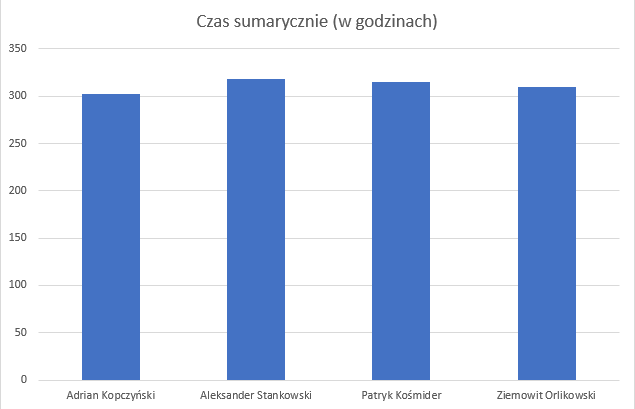
\includegraphics[width=1.0\textwidth]{images/timesheet_chart.png}
    \caption{Wykres godzinowego nakładu prac poszczególnych członków zespołu (opracowanie własne)}
    \label{img:timesheet_chart}
\end{figure}
\section{Zakres prac poszczególnych członków zespołu}
\par
Porjekt zrealizowano w 4 osobowym zespole, w którym każdy z członków miał przypisaną umowną rolę z jasnym zakresem obowiązków.
Takie rozwiązanie pozwoliło na wykorzystanie w pełni umiejętności wszystkich twórców oraz gwarancję ukończenia systemu w zaplanowanych ramach czasowych oraz na wysokim poziomie jakości.
\subsection{Adrian Kopczyński}
\par
W zespole pełniłem funkcje związane z zarządzaniem zespołem, projektem, procesami czy zapewnieniem jakości i testowaniem.
Jako kierownik zespołu byłem także przedstawicielem grupy odpowiedzialnym m.in. za komunikację zewnętrzną czy organizację zespołu projektowego.
\par
Na początku prac wytworzyłem dokumenty tj. Karta Projektu czy Dokument Założeń Wstępnych.
Byłem prowodyrem specyfikacji wymagań na system, tworząc przystępny system przechowywania wymagań z podziałem na: Identyfikator, Typ, Priorytet(MoSCoW), Treść Wymagania, Zmiany w treści, Status, Uwagi oraz Wymagania powiązane.
Podczas tego procesu upewniałem się, że każde z wymagań jest atomowe i testowalne (w miarę możliwości) oraz jest zrozumiałe stosując dobre praktyki tworzenia wymagań systemowych.
Po zakończeniu stworzyłem dokument Specyfikacja Wymagań Systemowych, który aktualizowany był na bieżąco w przypadku jakichkolwiek zmian.
Pełniłem również rolę właściciela produktu wskazując kierunek aplikacji, walidację przypadków użycia czy przepływy czynności wykonywanych w systemie.
W celu przybliżenia wizji systemu czy przypadków użycia utworzyłem opisową logikę biznesową, która była suplementem dla zespołu przed formalizacją wymagań i wyznaczała kierunek przepływów akcji w systemie.
Aby sformalizować tę wizję stworzyłem wizualizacje i diagramy używając języka UML, przedstawione w niniejszym dokumencie.
\par
Prowadziłem cotygodniowe spotkania zespołu zbierając statusy każdego z członków, próbując rozwiązać problemy oraz dokumentowałem przebieg spotkań w postaci notatek dostępnych dla wszystkich członków zespołu w wydzielonym folderze.
Utworzyłem przestrzeń na portalu Jira oraz zarządzałem strukturą zadań czy ich szablonami oraz byłem jedną z osób integrujących go z serwisem \gls{GitHub}.
Dbałem także o to, żeby zadania były odpowiednio traktowane poprzez walidację połączonych \gls{Epik}ów, etykiety czy zawartość samego zadania.
Byłem odpowiedzialny za ustalanie priorytetów zespołu, tworzeniu predykcji w oparciu o statusy oraz aktualizowanie harmonogramu projektu.
W ramach komunikacji przygotowywałem listy z pytaniami lub niejasnościami odnośnie samego procesu tworzenia pracy czy wymaganymi formalnościami oraz organizowałem spotkania z promotorem w celu ich wyjaśnienia.
Tworzyłem także \gls{mockup}'y dla interfejsu użytkownika.
\par
Przez cały czas trwania projektu byłem osobą dbającą o zapewnienie jakości wytwarzanego oprogramowania stosując dobre praktyki branżowe.
W fazie testowania byłem odpowiedzialny za przeprowadzanie testów \gls{E2E}, raportowaniu wyników, zgłaszaniu defektów oraz zarządzania ich cyklem życia.
W czasie trwania projektu byłem także odpowiedzialny za tworzenie niniejszego dokumentu oraz redakcję i kontrolę treści dotyczącej architektury systemu.
\subsection{Aleksander Stankowski}
\subsection{Patryk Kośmider}
\subsection{Ziemowit Orlikowski}